\documentclass[a4paper,11pt,english]{report}
\usepackage[utf8]{inputenc}
% Standard stuff
\usepackage{amsmath,graphicx,varioref,verbatim,amsfonts,geometry}
% colors in text
\usepackage[usenames,dvipsnames,svgnames,table]{xcolor}
% Hyper refs
\usepackage[colorlinks]{hyperref}
\usepackage{algorithm}
\usepackage{algpseudocode}
\usepackage{pifont}


% Document formatting
\setlength{\parindent}{0mm}
\setlength{\parskip}{1.5mm}

% Color scheme for listings
\usepackage{textcomp}
\definecolor{listinggray}{gray}{0.9}
\definecolor{lbcolor}{rgb}{0.9,0.9,0.9}
\makeatletter
\def\BState{\State\hskip-\ALG@thistlm}
\makeatother

% Listings configuration
\usepackage{listings}

\lstset{
  backgroundcolor=\color{lbcolor},
  tabsize=4,
  rulecolor=,
  language=python,
  basicstyle=\scriptsize,
  upquote=true,
  aboveskip={1.5\baselineskip},
  columns=fixed,
  numbers=left,
  showstringspaces=false,
  extendedchars=true,
  breaklines=true,
  prebreak = \raisebox{0ex}[0ex][0ex]{\ensuremath{\hookleftarrow}},
  frame=single,
  showtabs=false,
  showspaces=false,
  showstringspaces=false,
  identifierstyle=\ttfamily,
  keywordstyle=\color[rgb]{0,0,1},
  commentstyle=\color[rgb]{0.133,0.545,0.133},
  stringstyle=\color[rgb]{0.627,0.126,0.941}
}

\newcounter{subproject}
\renewcommand{\thesubproject}{\alph{subproject}}
\newenvironment{subproj}{
  \begin{description}
  \item[\refstepcounter{subproject}(\thesubproject)]
  }{\end{description}}

\newcommand{\mychapter}[2]{
  \setcounter{chapter}{#1}
  \setcounter{section}{0}
  \chapter*{#2}
  \addcontentsline{toc}{chapter}{#2}
}

% Lettering instead of numbering in different layers
% \renewcommand{\labelenumi}{\alph{enumi}}
% \renewcommand{\thesubsection}{\alph{subsection}}

% opening
\title{A journey to another planet}
\author{Aram Salihi}
\begin{document}
\begin{flushright}
  \small 5.~November, 2016
\end{flushright}
\vspace{10mm}

\begin{center}
  \vspace{5mm}
  \huge A journey to another planet
\end{center}
\vspace{3mm}
\begin{center}
  \includegraphics[scale = 1.3]{uio.png}
\end{center}
\vspace{3mm}
\begin{center}
  \author{Aram Salihi}
  \large  By: Aram Farhad Salihi\\ 
  \vspace{5mm}
  \large Username: arams\\
  \vspace{3mm}
 
  \huge Institute of Theoretical Astrophysics
\\
  University of Oslo\\
    \vspace{5mm}
    \huge AST1100
\end{center}
\vspace{3mm}

\clearpage
\tableofcontents
\newpage

\section{Acknowledgements}
 Firstly I would like to sincerely express my gratitude to my supervisor, Robert
Hagala, for guiding and answering my questions throughout this project, even though
he was often quite busy. I would also like to express my gratitude to my Professor
in "AST1100, A Introduction To Astrophysics ", Frode Hansen, for giving fun and
knowledgeable lectures.

I also want to thank my fellow students and friends, Gunnar Lange, Daniel
Heinesen and Frederik L. Mellbye, for our partial cooperation, as well as introducing me to  new ideas.

\section{Introduction}
I have been given a random seed, 23078, this seed represents my
solar system, which consists of 1 star and 9 planets. I have decided to travel to
the neighbouring planet, which I called G23 in this project. To travel to this
planet we need an engine capable of reaching my planet's escape velocity,
but as well as making maneuvers during the trip. With several simple
boxes with holes in them, the engine is capable of doing these tasks.


In order to plan my satellite's
trajectory, I need to know the motion of my solar system.  Using Newton's
second law and his law of gravity, I can predict the motion of the planet's.  I 
now have an engine and an understading of how my solar system behaves,
I can then give
a little extra boost at a certain time, which will be enough to take off from
my homeplanet and fly to G23.

When  the satellite is in deep space, it is crucial to know what the position and
velocity of the satellite is, to fix this issue I have implemented an orientation
software. As time passes the satellite approaches G23, thereafter making an
injection burn
 to enter G23's orbit. The satellite is now in a position where it can take
 orbital pictures
and videos, however I am not yet finished, I want to explore the planet. With
some simple physics and statistics, I can then find out what the atmosphere consists
of, because as the satellite approaches G23,  it gets warmer due to the drag forces in the
atmosphere; I need to carefully direct it towards G23's surface
so it does not crash or burned.

As the satellite approaches a safe height,  so it can detatch its probe, the
probe will approach G23's surface, and at some altitude it will approach
terminal velocity
(stops accelerating), and then  deploy its parachute. As the lander have landed
on the surface it will take pictures and send it back to its homeplanet.



\newpage
\mychapter{2}{Method}
\subsection{Engine}
\subsubsection{A simple model:}
In the introduction I briefly explained how to build a rocket engine, in this
section I will explain it in more detail. As I mentioned, the engine consists of
several cubes with length \(d\).
\begin{figure}[h]
  \centering
  \includegraphics[scale = 0.5]{Kube.png}
  \caption{A example on how the cube will look like}
\end{figure}
\\
Inside this cube there will be 100 000 random positioned hydrogen molecules,
with Gaussian distributed velocity (I will explain this in more detail in the
next section). In order to accelerate the rocket, I need to a implement a hole so
the molecules can escape (Change in momentum will accelerate the rocket) the
cube. This hole is located at the bottom of the cube, (\(z  = 0\)), in the
interval
\begin{align}
  \frac{d}{4} \le x,y \le \frac{3d}{4}
\end{align}
When a hydrogen molecule have a \(z\) component less or equal to \(0\),( \(z \le
0\)), it will
escape through this hole. I will then replace this hydrogen molecule on the
top side of the box with a random \(x,y\) position. I have implemented a sensor
which counts amount of particle escaped, escaped momentum, pressure inside the
box.
\newpage
\subsubsection{Motion of the Molecules:} As I mention in the previous section
the hydrogen molecules are uniformly random positioned in the interval
\(x,y,z \in [0,L]\) with a gaussian distributed velocity. The motion of the 
molecules is described with Maxwell-Boltzmann distribution (skriv referanse
her, Part1A)
\begin{align}
  P(\bold{v}) = (\frac{m_{H_{2}}}{2\pi
  k_{b}T})^{\frac{3}{2}}e^{-\frac{m_{H_{2}}v^{2}}{2k_{b}T}} =( \frac{1}{2\pi
  \sigma^{2}})^{\frac{3}{2}}e^{-(\frac{v_{x}^{2} + v_{y}^{2} + v_{z}^{2}}{2\sigma^{2}})}
\end{align}
due to large amount of particles, constant and high temperature, the most probable speed
is \\expressed as
\begin{align}
  v = \sqrt{\frac{k_{b}T}{m_{H_{2}}}}
\end{align}
I can then also use expression (2.3) to define it as the standard deviation,
\(sigma\), in expression (2.2). The speed of the molecules will now be in the
range \([0, \sqrt{\frac{k_{b}T}{m_{H_{2}}}} ]\).
\subsubsection{Pressure and Momentum inside the cube:} First of all to simplify some
problem for example change in momentum I will assume there is no
interaction/collisions between the molecules, only elastic collision
\footnote{An elastic collision is a direct collision between two object where
  the total momentum and kinetic energy is consered.} between the walls. To a
have fully functioning engine the pressure inside have to be stable. To find
the pressure, I will look at the
change in 
momentum when the molecules are colliding with the wall. The change is then (referanse fra part1A notater)
\begin{align}
 p_{\mathrm{wall}} =  \sum_{j = 1}^{K}2m_{\mathrm{H_{2}}}v_{\mathrm{x,j}} =
  2\Delta p_{x}
\end{align}
Since I know the change in momentum, I can find the pressure exerted on the
wall. The pressure is propotional to the force exerted on the wall in a time
interval \(\Delta t\). The pressure is then mathematically described as 
\begin{align}
  P =  \frac{2\Delta p_{x}}{A\Delta t}
\end{align}
From the previous section I defined the temperature to \(T\) (constant), and
the highly probable speed is defined to be \(\frac{k_{b}T}{m_{H_{2}}}\), the
change in
momentum on the wall is approximated to be constant therefore the pressure will also
be constant.
\newpage
\subsubsection{Totalfroce and thrust from the engine:} To find the totalforce from the
engine, I need to know how many cubes I need in order to accelerate to the
\(\Delta v\) I want. Newton's second law states that
\begin{align}
  \sum_{j}F_{j} = ma
\end{align}
In this situation there is only one force, \(F_{engine}\), which describes the
totalforce from all the cubes. To simplify the problem, I assume that the
satellite have
reached the \(\Delta V\), and all the fuel is used up. 
\begin{align}
  F_{\mathrm{cube}}n_{\mathrm{cube}} = m_{r}\frac{\Delta V}{\Delta t_{\mathrm{launch}}}
\end{align}
solving with respect to \(n_{\mathrm{cube}}\), I will get
\begin{align}
  n_{\mathrm{cube}} = \frac{m_{r}\Delta V}{F_{\mathrm{cube}}\Delta t_{\mathrm{launch}}}
\end{align}
\(\Delta t_{\mathrm{launch}}\) describes how long it take to burn up all the
fuel. The totalforce is therefore force per cube multiplied with number of
cubes. To find out how effective a rocket engine is, I have to look at the
thrust velocity. Thrust velocity is how much mass is expunged out of the engine per time. To find
thrust, I can look at the force from one cube, which I can express it as
\begin{align}
  F_{cube} = \frac{p_{e}}{\Delta \tau}n_{e}
\end{align}
where \(p_{e}\) is the momentum escaped from the engine defined as
\(2m_{H}\mu\), where \(\mu\) is the thrust velocity (I have multiplied with 2 because it
is hydrogen molecules and not atoms), and \(n_{e}\) is the number of molecules
escaped from the cube per \(\Delta \tau = 10^{-9}\). Expresssion (2.9) can then be expressed
as
\begin{align}
  F_{cube} = \frac{2m_{H}\mu}{\Delta \tau}n_{e}
\end{align}
solving for \(\mu\)
\begin{align}
  \mu = \frac{F_{cube}\Delta \tau}{2 m_{H}n_{e}}
\end{align}
Expression (2.11) defines how effective the rocket engine is.
\newpage
\subsection{Fuel Amount}
To make the project more realistic the rocket engine needs fuel to function. I have
found two ways to calculate the amount of fuel I need throughout the entire trip.
\paragraph{Method 1: Analytical Solution}:  Newton's Second Law states that
force is proportional to acceleration (multiplied with an constant mass, \(m\)).
Consider a situation where the mass changes as  time passes in the \(z\) direction (upwards)
\begin{align}
  \sum_{j}F_{j}^{ext} = (\Delta m_{f} + m_{r})a 
\end{align}
where \(\Delta m_{f}\) describes the changing mass, which in this case is the
amount of fuel used, and \(m_{r}\) describes the satellite's mass. Acceleration is the time
derivative of the velocity, \(a = \frac{dv}{dt}\), expression (2.12) can be
expressed in terms of deltas
\begin{align}
  \sum_{j}F_{j}^{ext} = \frac{(\Delta m_{f} + m_{r})\Delta v}{\Delta t} =
  \frac{\Delta p}{\Delta t}
\end{align}
where \(\Delta p\) is the change in momentum. The interesting part is how 
momentum changes with time. To make certain steps easier, I've assumed that I
am starting
at a time \(t\) with fuel \(\Delta m\), and that I've reached burnout at time
\(t + \Delta t\).
The momentum at time \(t\) is then \(p(t) = \Delta m\mu_{e}
+ m_{r}v\)\\ (\(\mu_{e}\) is the velocity at which the particle is expunged out of the
engine, this is a constant that also defines how efficient the engine is).
At time \(\Delta t + t\) the momentum has changed to \\
\(p(\Delta + t) = m_{r}(v+ \Delta v)\), the total change \(\Delta p\) is then
\begin{align}
  \Delta p = p(\Delta t + t)-p(t) = m\Delta v -\Delta m\mu_{e}
\end{align}
By inserting expression (2.14) in to (2.13) and taking the limit when \(\Delta t \to
0\), expression (2.13) can then mathematically be described as
\begin{align}
  \sum_{j}F_{j}^{ext}  + \mu_{e}\frac{dm_{f}}{dt} = m_{r}\frac{dv}{dt}
\end{align}
This equation is called Tsiolkovsky's rocket equation. I now have an equation
with a time dependent mass.  I can assume that the net external force
\(\sum_{j}F_{j}^{ext} = 0\) for simplicity's sake I will not include gravity
(I will discuss this statement in depth in
the discussion part). Expression (2.15) is now a separable differential
equation, of the form
\begin{align}
  \mu_{e}dm = mdv
\end{align}
As I derived previously, \(\mu_{e}\) is a constant which can be defined as
\begin{align}
  \mu_{e} = \frac{F\Delta \tau}{2n_{e}m_{H}}
\end{align}
where \(F\) is the force per box, \(n_{escaped}\) is the number
of hydrogen molecules that have escaped per box,  and \(m_{H}\) is the mass of a
single hydrogen atom (that's why I multiplied it by 2), and \(\Delta \tau = 1ns\)
Going back to expression (2.16), and integrating both sides with
integration limits, it follows that:
\begin{align}
  \int_{ m_{r} + m_{r}}^{m_{r}}\frac{dm}{m}= \int_{0}^{\Delta
  V}\frac{dv}{\mu_{e}}
\end{align}
\vspace{3mm}
\begin{align}
  \ln{\frac{m_{r}}{m_{r} + m_{f}}} = \frac{\Delta V}{\mu_{e}}
\end{align}
Solving with respect to \(m_{f}\), the equation for the amount of fuel I need
throughout the trip is given by
\begin{align}
  m_{f} = m_{r}(e^{{-\frac{\Delta V}{\mu_{e}}}} -1)
\end{align}
\paragraph{Method 2: Numerical Solution:} In order to do this numerically I will
solve a differential equation of the form
\begin{align}
  \frac{d^{2}r}{dt^{2}} = \frac{F}{m_{r}+m_{f}}
\end{align}
where I guess how much fuel (\(m_{f}\)) I need, and I defined 
\(F = \frac{\Delta p_{e}}{\Delta t_{period}}n_{box}\) in the part where I talked about
the engine. I will use the numerical Euler-Cromer method
\begin{align*}
  a_{i}(r,t)
  \\
  v_{n+1} = v_{n} + a_{i}\Delta t
  \\
  x_{n+1} = x_{n} + v_{n+1}\Delta t
  \\
  \Delta t =  \frac{t}{N}
\end{align*}
where \(t\) is the launch period, and \(N\) reperesents the number of iterations. For
every timestep I will subtract  a mass of magnitude
\(m_{escaped} = \frac{m_{H_{2}}n_{escaped}n_{boxes}}{\Delta t_{period}}\), where I
still use \(\Delta t_{period} = 1ns\). I have also implemented an if test which
breaks the for loop if the rocket has reached the \(\Delta v\) I want or used up
all of its fuel. The algorithm will then look like this
\begin{algorithm}
  \caption{Fuel finder}
  \label{CHalgorithm}
  \begin{algorithmic}[1]
    \For{i in xrange(N-1):}
    \\
    \State \(a = \frac{F}{m_{f} + m_{r}}\)
    \State \(v_{i + 1} = v_{i}  + a_{i}\Delta t\)
    \State \(x_{i + 1} = x_{i} + v_{i + 1}\Delta t\)
  \State \(m_{f} -= m_{\mathrm{escaped}}\) 
    \EndFor
  \end{algorithmic}
\end{algorithm}


\newpage
\subsection{Motion of the Solar System:} To make things more realistic, it
is crucial to know the motion of the planet you are traveling to, but also the
rest of the solar system. The reason being cost; it is not cheap to send a satellite out
to another planet, but as well because of avoiding gravity from certain planets
or using gravity assist to accelerate and guide the satellite to the destination.
As I mentioned in the introduction, to predict the motion of
the solar system I am going to use Newton's Second Law, his Law of Gravity,
and numerically solve the following ordinary differential equation for an
\(N\)-body system

\begin{align}
  m_{p}\frac{d^{2}\bold{r}}{dt^{2}} = - \frac{Gm_{p}m_{s}}{r^{2}}\frac{\bold{r}}{r}
\end{align}
where \(\frac{\bold{r}}{r}\) is a two dimensional unit vector in the  \(xy\) plane, and \(\bold{r}\)
is the position vector relative to the star defined as \(\bold{r}_{rel} =
\bold{r}_{planet} - \bold{r}_{star}\). I will then assume that since the star
is so massive compared to the planets, the star would not move. So I set
\(\bold{r_{star} = \bold{0}}\). The numerical method I used was the Euler-Cromer
method, but I could use aslo Leap-Frog (I will discuss in the discussion part why I
did not use it). The algorithm for solving this problem
\begin{algorithm}
  \caption{Solving N-body system}\label{euclid}
  \begin{algorithmic}[1]
    \For{for i in xrange(N-1)}:
    \For{for j in xrange{(Number of planets)}}:
    \\
    \State \(\bold{r^{rel}_{i+1,j}} = \bold{r}^{planet}_{i,j} - \bold{0}\)
    \\
    \State \(a_{i,j} = (\frac{M_{star}G}{(r^{rel}_{i,j})^{3}})\bold{r}^{rel}\)
    \\
    \State $v_{i+1,j} = v_{i,j} + a_{i,j}\Delta t$.
    \\
    \State \(x_{i+1,j} = x_{i,j} + v_{i+1,j}\Delta t\)
    \EndFor
    \EndFor
  \end{algorithmic}
\end{algorithm}
\\
But in reality, so will the center of mass of the star slighty move in realtion
to the planets. This can be shown mathematically and by observation.
\subsection{Motion of the Star:}
\subsubsection{Observation} From observation one can show that the light
intensity slightly vary, this is due to slight movements. If we look at the
spectrum of the star, one will notice a slight periodic shift. One can find
this shift by using the doppler effect
\begin{align}
  \frac{v_{rel}}{c} = \frac{\Delta \lambda}{\lambda_{0}}
\end{align}
In most cases these shift are caused by exoplanets  orbiting around the star,
causing the star move slight around its center of mass.

\subsubsection{Theoretical:}
I define the center of mass of the star to be \(\bold{R}_{star}\), and the
velocity is,
\(\bold{V}_{star} = \frac{d\bold{R}_{star}}{dt}\). I will now assume that the
total momentum and energy of the solar system is  conserved
\begin{align}
  \sum_{k =1}^{N}\bold{P}_{j} = \bold{0}
\end{align}

\(\bold{P}_{j}\) is momentum. Expression (2.24) can be expanded to
\begin{align}
  M_{star}\bold{V}_{star}  = \sum_{k=1}^{N-1}\bold{P}_{j}
\end{align}
The left hand side is the momentum of the star, and on the right hand side is
the momentum of all the planets orbiting around the star. Dividing by the mass
of the star, I will get the following expression
\begin{align}
  \bold{V}_{star} = \frac{ \sum_{k=1}^{N-1}\bold{P}_{j}}{M_{star}}
\end{align}
Expression (2.26) shows that; planets orbiting around a star will cause the
star to move slight around its center of mass. 
\subsection{Planet G23:}
\subsubsection{Surface Temperature of G23}
I have now the knownledge of my solar systems
motion, but I need further information about the planets. The most important
one is the surface temperature. This temperature reveals if the planet is
habitable planet or not. Looking at the energy recevied from the star
\begin{align}
  Fd\hat{A}= \frac{dE}{dAdt}d\tilde{A} = \frac{R_{*}^{2}\sigma T_{*}^{4}}{a^{2}}d\tilde{A}
\end{align}
 The differential
\(d\tilde{A}\) is the area that absorbs the energy for the star. Assuming that
the planet is black body, the planet will then follow Stefan-Boltzmann law
\begin{align}
  F = \sigma T^{4}
\end{align}
From Stefan-Boltzmann law I can then find the energy sent out by the planet.
The energy recevied from the star has to equal the energy the planet are
sending out
\begin{align}
  E_{\mathrm{inn}} = E_{\mathrm{out}} 
\end{align}
expressing equation (2.29) as
\begin{align}
  F_{\mathrm{out}}dA_{\mathrm{planet}} = \frac{R^{2}_{*}\sigma T^{4}_{*}}{a^{2}}d\tilde{A}
\end{align}
integrating with respect to area, I will get
\begin{align}
  4\pi r^{2}_{\mathrm{planet}}\sigma T_{\mathrm{planet}}^{2} = \pi
  r_{\mathrm{planet}}^{2}  \frac{R^{2}_{*}\sigma T^{4}_{*}}{a^{2}}
\end{align}
The surface temperature of an arbitrary planet is (remember that \(r_{planet}\)
is the radius of the planet)
\begin{align}
  T_{\mathrm{Planet}} = T_{*}\sqrt{\frac{R_{*}}{2a}}
\end{align}
This explain the surface Temperature of a planet with no green house effect.
I assume that habitable planet have a sufrace temperature in the interval
\([260K, 390K]\). Calculating the surface temperature for G23, I will get that
the temperature is \(T_{\mathrm{G23}} = 273,38K\) which means it is habitable.
Expression (2.27) and (2.28) is aquired from
\footnote{AST1100 lecture notes Part1D, author Proffesor Frode Hansen}

\subsubsection{Planning the journey to G23:} Now it is the time to launch the satellite
in to deep space toward G23. In order to get to G23 with the 
smallest fuel consumption as possible, I will do a transfer orbit around my
star and to G23.
The reason is the gravity assist from the star, this effect will accelerate the
satellite, and give the right path to G23 with minimal correction boost/burn. I am
going to  use Hohmann transfer\footnote{\url{https://en.wikipedia.org/wiki/
    Hohmann_transfer_orbit}\\
  and\\
  \url{https://ocw.mit.edu/courses/aeronautics-and-astronautics/16-07-dynamics-fall-
    2009/lecture-notes/MIT16_07F09_Lec17.pdf}}.  When the satellite takes a
Hohmann transfer orbit, it goes from a lower orbit to a higher circular orbit.
This is a elliptic orbit which touches the initial orbit at perihelion and at
aphelion (the final destination). In this proccess the total kinetic energy and
angular momentum is fully conserved.
\begin{figure}[h]
  \centering
  \includegraphics[scale = 0.5]{hohmann-transfer.jpg}
  \caption{This figure illustrates Hohmann transfer orbit}
\end{figure}
\\
  The \(\Delta v\) required  to get to G23's orbit is
  mathematically described as
  \begin{align}
    \Delta V = \sqrt{\frac{m_{star}G}{r_{1}}}(\sqrt{\frac{2r_{2}}{r_{1} + r_{2}}} - 1)
  \end{align}


to make the transfer orbit most efficient, I have to launch the satellite at a
certain angle and at certain time when my homeplanet and G23 is aligned. To
find this angle I will use the expression
\begin{align}
  \alpha = \pi[1 - \frac{1}{2\sqrt{2}}\sqrt{(\frac{r1}{r2} + 1)^{3}} ]
\end{align}
and to find the time when this event happens I have made a
algorithm which calculates it

 The time it will take to reach G23 is calculated from the expression
\begin{align}
  t_{H} = \pi \sqrt{\frac{(r_{1} + r_{2})^{3}}{8GM_{star}}}
\end{align}

\begin{algorithm}
  \caption{Time align finder algorithm}
  \label{CHalgorithm}
  \begin{algorithmic}[1]
    \State \(\alpha =\pi[1 - \frac{1}{2\sqrt{2}}\sqrt{(\frac{r1}{r2} + 1)^{3}} ] \)
    \State \(c = 0\)
    \State \(\phi = 0\)
    \While{ \(c < N\):}
    \\
    \State \(\phi = \arccos{(\frac{\bold{r_{home}}\cdot\bold{r_{G23}}}{|\bold{r_{home}}|
        |\bold{r_{G23}}})}|\)
    \State \(t = times[c]\)
    \State \(c += 1\)
    \If{ \(\phi \le \alpha\):}
  \State break
  \EndIf
  \EndWhile
  \State return \(\phi\), \(t\)
  \end{algorithmic}
\end{algorithm}
\subsubsection{Solarpanels:} When the satellite is in deep space, and not using
fuel to function, and to function it has to rely on a energy source. To solve
this problem I can use energy from the light sent out by star (or other stars),
which means the satellite need solar panels, these panels have a efficieny of
\(12\%\), and a power of \(P = 40W\) . The question is how big these solar
panels have to be. The area of
the solar panels can by found from flux recieved from my star
\begin{align}
  F = \frac{dE}{dAdt}
\end{align}
Multiplying with the area of the solar panel, the power can be expressed as
\begin{align}
  FA_{panels} = \frac{dE}{dAdt}A \to P = \frac{L}{4\pi d^{2}}A_{panels}
\end{align}
where \(L\) is the luminosity is expressed \(4\pi R_{*}^{2}\sigma T^{4}_{*}\).
The solar panel only have a efficiency of \(12\%\), the power is then \(\frac{P}{0.12}\).
Solving with respect to A
\begin{align}
  A_{panel} = \frac{d^{2}P}{0.12\sigma T^{4}_{*}R^{2}}
\end{align}
The area of the solar panels needed are expressed with expression (2.38)
\newpage
\subsection{Orientation, Position and Velocity:}
While the satellite is in deep space, it's very important to know
its orientation, position and the velocity. To find this out I have one method
to each of these issues.
\subsubsection{Orientation:} To find the orientation of my satellite,  I can compare existing
picture of the sky or my path with pictures taken from the satellite. To do
this I will do 360 projection of the sky and compare these pictures with the
existing ones, and from that I can find my orientation angle.
I will use the method stereographic projection. This method 
maps each position on the sphere, denoted by
\(\theta\) and \(\phi\), onto a point on the tangent plane of the surface about
some point \(\theta_{0}, \phi_{0}\), the opposite is  also possible.

\begin{figure}[h]
  \centering
  \includegraphics[scale = 0.75]{stereoprojection.png}
  \caption{This picture illustrates how stereopgraphic works. It takes a
    spherical picture makes into a flat picture, \((\phi_{0}, \theta_{0})\)
    \(\to\) \((x_{\mathrm{picture}}, y_{\mathrm{picture}})\)}
  \end{figure}
I am going to define the points in the tagnet plane as \(x_{\mathrm{picture}}\)
and \(y_{\mathrm{picture}}\). Further I am going to use \((\phi - \phi_{0})_{max} =
\frac{\alpha_{\phi}}{2}\) and \((\theta - \theta_{0})_{max} =
\frac{\alpha_{\theta}}{2}\) , these meassures the difference between the outer edge
and the midtpoint in the picture measurred with the angles \(\phi, \theta\).
 Using the equation
\begin{align}
  x_{max/min} = \pm \frac{2\sin{\frac{\alpha_{\phi}}{2}}}{1+
  \cos{\frac{\alpha_{\phi}}{2}}}
  \\
  y_{max/min}=  \pm \frac{2\sin{\frac{\alpha_{\theta}}{2}}}{1+
  \cos{\frac{\alpha_{\theta}}{2}}}
\end{align}
From these equations I can find the maximum and the minimum pixel placement in
the picture at the midpoint and at the outer edge. Defining \(x_{max/min}\) and
\(y_{max\min}\) as a interval \([x_{min}, x_{max}]\) and \([y_{min},
y_{max}]\), using values from these interval I can find 
the spherical positions \(\theta\) and \(\phi\).Using the equations

\begin{align}
  \theta = \frac{\pi}{2}  -\arcsin{(\cos{c}\cos{\theta_{0}} + \frac{y_{picture}
  \sin{c}\sin{\theta_{0}}}{\rho})}
\end{align}
\begin{align}
  \phi = \phi_{0} +
  \arctan{(\frac{x_{picture}\sin{c}}{\rho\sin{\theta_{0}}\cos{c} -
  y_{picture}\cos{\theta_{0}}\sin{c}})}
\end{align}
\begin{align}
  \rho = \sqrt{x^{2}_{picture} + y^{2}_{picture}}
\end{align}
\begin{align}
  c = 2\arctan{\frac{\rho}{2}}
\end{align}
when the angles are found, I am sending these angles to a module which makes
the angles into pixel with RGB colors. Putting the pixels together into a
matrix, I can now compare these 360 pictures with the existing picture (In this case I
have used a \(640\times480\) matrix). To find the picture which is approximated
to the existing one, I can use least squares method
\begin{align}
  Q = \sum_{j}^{360}(\mathrm{Existing} - \mathrm{Projection}[j])^{2}
\end{align}

These equations and expression is aquired from 
\footnote{Part4 AST1100 Satellite project, author Proffesor Frode
  Hansen}. 

\subsubsection{Position finder:} To find the satellites position, I will
implement a radar. This radar have the property to find the position \(x,y\) of the
sallite by using three referance points in space, since I already know the position
of the planets and the star at all time, I can use the planets and the star
positions as referance points. I can then create three  large circle around these
points where the radius is the distance between the satellite and the referance
point.
This will then give me three circle equation which I need to solve
\begin{align}
  x^{2} + y^{2} = d_{1}^{2}
  \\
  (x- x_{2})^{2} + (y - y_{2})^{2} = d_{2}^{2}
  \\
  (x - x_{3})^{2} + (y - y_{3})^{2} = d_{3}^{2}
\end{align}
The first equation represents the position of the star with a distance
\(d_{1}\) to the satellite. The other two equation reperesents an arbitrary
planet with a distance \(d_{2}\) and \(d_{3}\) to the satellite. I am now
interested to find \(x,y\).  multiplying out the parantheses in expression
(2.47) and (2.48),  so I get
\begin{align}
  x^{2} + y^{2} = d_{1}^{2}
  \\
  x^{2} - 2xx_{2} + x_{2}^{2} + y^{2} - 2y_{2}y + y^{2} = d_{2}^{2}
  \\
  x^{2} - 2xx_{3} + x_{3}^{2} + y^{2} - 2y_{3}y + y^{2} = d_{3}^{2}
\end{align}
Inserting \(x^{2}\) from expression (2.49) into expression (2.50) and (2.51), I
will get
\begin{align}
  2x_{2}x + 2yy_{2} = d_{1}^{2} - d_{2}^{2} + x_{2}^{2} + y_{2}^{2}
  \\
  2x_{3}x + 2yy_{3} = d_{1}^{2} - d_{3}^{2} + x_{3}^{2} + y_{3}^{2}
\end{align}
expression (2.52) and (2.53) and can be written as a matrix equation
\begin{align}
  \begin{pmatrix}
    x_{1} & y_{1}
    \\
    x_{2} & y_{2}
  \end{pmatrix}
            \begin{pmatrix}
              x
              \\
              y
            \end{pmatrix}
  =
  \begin{pmatrix}
    \frac{(d_{1}^{2} - d_{2}^{2} + x_{2}^{2} + y_{2}^{2})}{2} \\
    \frac{(d_{1}^{2} - d_{3}^{2} + x_{3}^{2} + y_{3}^{2})}{2} 
  \end{pmatrix}
\end{align}
solving equation (2.54), I will find the \(x,y\) position of the satellite.
\subsubsection{velocity of the satellite:} To do maneuvers during the trip it
is crucial to know the velocity of the satellite. One way to find the velocity
is to look at the wavelength at a certain angle \(\phi_{1}\) and \(\phi_{2}\) from two distant
stars. When light travels a long
distance or if the satellite approaches a star, the light will be slightly shifted. 
This is the doppler effect.
\begin{align}
  \frac{v}{c} = \frac{\Delta\lambda}{H_{\alpha}}
\end{align}
where \(H_{\alpha} = 656.3nm\) is the non shifted light sent out by the
reference star, and
\(\Delta \lambda\) is the shift measured relative to my star. Using this I will
find out the velocity relative to my star and not the satellite. Receving the
same light beam, but meassuring another doppler shift, using this shift I
can meassure the velocity of the reference star relative to my satellite. The
velocity of my satellite is then expressed as
\begin{align}
  v_{satellite} = v_{\mathrm{refstar}\to\mathrm{star}} - v_{\mathrm{refstar}\to\mathrm{satellite}}
\end{align}
where
  \begin{align}
    v_{\mathrm{refstar}\to\mathrm{star}}  = \frac{\Delta \lambda}{H_{\alpha}}c
    \qquad
    v_{\mathrm{refstar}\to\mathrm{satellite}} =  \frac{\Delta \lambda_{\mathrm{satellite}}}{H_{\alpha}}c
  \end{align}
The expression on the left expresses the velocity of the reference star1
relative to my star. The expression on the right expresses the exact same but
relative to my satellite. I will now use the same on reference star2. The
velocity of my satellite is then given as; Described with Referance star 1
\begin{align}
  \bold{v}_{1} =  v_{satellite} = v_{\mathrm{refstar1}\to\mathrm{star}} -
  v_{\mathrm{refstar1}\to\mathrm{satellite}}
\end{align}
Described with Referance star 2
\begin{align}
  \bold{ v}_{2} =  v_{satellite} = v_{\mathrm{refstar2}\to\mathrm{star}} -
  v_{\mathrm{refstar2}\to\mathrm{satellite}} 
\end{align}
expression (2.58) and (2.59) is just a matrix equation, and it is given as
\begin{align}
  \begin{pmatrix}
    v_{x}\\
    v_{y}
  \end{pmatrix}
  = \frac{1}{\sin{(\phi_{1} - \phi_{2})}}
  \begin{pmatrix}
    \sin{\phi_{2}} & -\sin{\phi_{1}}\\
    -\cos{\phi_{2}} & \cos{\phi_{1}}
  \end{pmatrix}
                      \begin{pmatrix}
                        v_{1}\\
                        v_{2}
                      \end{pmatrix}
\end{align}
  solving this matrix equation, I will find the velocity of the satellite. 
  \subsection{Orbit around G23:}
\subsubsection{Minimal Distance}
When the satellite gets closer to G23 it have to
a injection burn. This injection burn occours when the satellite is at its
closest to the planet. I then need to know this distance. To find the distance
I can look at the ratio between of the force excerted on th satellite from G23
and the planet. The force from the star
\begin{align}
  F_{*} = \frac{m_{sat}M_{*}G}{R^{2}}
\end{align}
where \(R\) is the distance between satellite and the star. The force from G23
\begin{align}
  F_{G23} = \frac{m_{sat}M_{G23}}{r^{2}}
\end{align}
finding the ratio, and defining the magnitude as \(k\), I will get the
expression
\begin{align}
  \frac{R^{2}_{*}m_{G23}}{r^{2}M_{*}} = k
\end{align}
Solving expression (2.63) with respect to the distance between G23 and the
satellite, \(r\), gives me
\begin{align}
  r = \sqrt{\frac{R_{*}m_{G23}}{M_{*}k}}
\end{align}
Using expression \(2.64\) I can find out the distance needed to do a injection
burn.
\subsubsection{Correction Boost/Burn:} In general to get close enough to the planet,
one has to do an correction boost/burn. A correction boost is a boost/burn which changes
the direction of the velocity vector with increasing or decreasing speed, it
depens on the situation. I will now define the correction burn as a some scalar
factor \(Q\) multiplied with the position vector.
\begin{align}
  \bold{v_{burn}} = -Q\frac{\bold{r}}{|\bold{r}|}
\end{align}
Since I know the position of G23 at all time, I will define the position vector
to the satellite relative to G23 as
\begin{align}
  \bold{r_{rel}} = \bold{r_{sat}}(t) - \bold{r_{G23}}(t+\Delta t)
\end{align}
Expression (2.66) will then ensure that I boost/burn towards G23. If the scalar
factor \(Q\) is negative, it will be a boost toward the planet, and positive it
will be a burn.

\subsubsection{Injection Boost:} After reaching the closest distance to G23, I
can finally do a injection boost in to a stable circular orbit. To find the
velocity needed in order to achieve a stable circular orbit, I have to look at
Newton's second law expressed with sentripetal accelartion, \(a =
\frac{v^{2}_{so}}{|\bold{r}|}\)
\begin{align}
  F = m(\frac{v^{2}_{SO}}{|\bold{r}|})
\end{align}
At this distance the dominating force is from G23, I can therefore neglect
neighbouring planet and the star. Using Newton's law of gravity, I can solve
expression (2.67) with respect to \(v_{so}\). I will then get the expression
\begin{align}
  v_{so} = \sqrt{\frac{m_{G23}G}{|\bold{r}_{rel}|}}
\end{align}
But even though I have the value of the velocity I need, I still need the
change in velocity relative to G23
and \(v_{so}\) have to be a velocity vector and not a scalar.
To make expression \(2.68\) in to a vector, I can place G23 in the center in a
another coordinate system, and find a angle \(\theta\) between the satellite
and G23. The angle \(\theta\) is only the coordinates of \(\bold{r_{rel}}\)
expressed in polar coordinates. To find \(v_{so}\), I can express the position
vector in polar coordinates
\begin{align}
  \bold{r_{rel}} = |\bold{r_{rel}}|(\cos{\theta}, \sin{\theta}) = |\bold{r_{rel}}|\hat{i}_{\theta}
\end{align}

Differentiating expression (2.69) at a time \(t + \Delta t\), the velocity
relative to G23 is given by
\begin{align}
  \frac{d}{dt}(|\bold{r}_{rel}|\hat{i_{r}}) = \frac{d}{dt}|\bold{r}_{sat} -
  \bold{r}_{g23}|\hat{i}_{r} + |\bold{r_{rel}}| \frac{d}{dt}\hat{i_{r}}
\end{align}
which gives me
\begin{align}
  \frac{d}{dt}(|\bold{r}_{rel}|\hat{i_{r}})  =  \frac{d}{dt}|\bold{r}_{sat} -
  \bold{r}_{g23}|\hat{i}_{r} + |\bold{r_{rel}}|\hat{i}_{\phi} 
\end{align}
here is \(\hat{i}_{r} = (\cos{\phi}, \sin{\phi})\) and \(\hat{i}_{\phi} =
(-\sin{\phi}, \cos{\phi})\). Assuming the distance \(|\bold{r_{rel}}|\) at a
time \(t+ \Delta t\) is constant, the term  \(\frac{d}{dt}|\bold{r}_{sat} -
\bold{r}_{g23}|\hat{i}_{r}= \bold{0}\). I have then the velocity at a time
\(t + \Delta t\)
\begin{align}
  \frac{d}{dt}(|\bold{r}_{rel}|\hat{i_{r}}) =  |\bold{r_{rel}}| \frac{d}{dt}\hat{i_{r}}
\end{align}
which is also the same as
\begin{align}
  \frac{d}{dt}(|\bold{r}_{rel}|\hat{i_{r}}) =
  -|\bold{r}_{rel}|\hat{i}_{r}\frac{d\phi}{dt} = |\bold{\omega} \bold{r}_{rel}|\hat{i}_{\phi}
\end{align}
The right handside of expression (2.73) is just \(v_{so}\). That means that
\begin{align}
  \frac{d}{dt}(|\bold{r}_{rel}|\hat{i_{r}}) =
  \sqrt{\frac{m_{G23}G}{|\bold{r}_{rel}|}}\hat{i}_{\phi} = \sqrt{\frac{m_{G23}G}{|\bold{r}_{rel}|}}
(-\sin{\phi},\cos{\phi})
\end{align}
The change in velocity from time \(t\) to \(t + \Delta t\) is expressed as
\begin{align}
  \Delta v = v_{so}\hat{i}_{\phi} - (\bold{v}_{sat} - \bold{v}_{planet}) =
  \bold{v}_{so}- (\bold{v}_{sat} - \bold{v}_{planet})
\end{align}
Using expression (2.75) the satellite manages to get into a stable orbit around G23.
\subsection{Analyzing the Atmosphere:}The satellite is now in orbit, Before the
satellite go to a lower orbit and  detatch its
landerprobe, I have to know what type of gas molecules the atmosphere consist of,
this is because of air resistance.
To find out what kind of gas molecule the atmosphere consist of, I will look at the
spectras. Assuming that I have a list of the noise,  wavelength and its flux sent out of
G23 atmosphere, I can create a model of the flux and compare it with the real
values. From previous section I know that, when a moving molecule emits
light, it will occour  doppler shift will occour.

Assuming that the
movement is caused by a temperature in the interval \(T \in [150k, 450k]\) and
I know that particle motion is Gaussian, I can
find the standard diviation of the doppler shift from a arbitrary gas molecule
\begin{align}
  \sigma = \frac{2\lambda_{center}}{c}\sqrt{\frac{k_{b}T }{m_{gas}}}
\end{align}
The wavelengths are centered around the arbsorption lines
\(\lambda_{center}\). Trying different  standard deviation, the
model of the flux can be expressed as
\begin{align}
  F^{model}(\lambda_{center}, \lambda,\sigma, F_{min},F_{max}) = F_{max} +
  (F_{min} - F_{max})e^{-\frac{(\lambda - \lambda_{center})^{2}}{2\sigma^{2}}}
\end{align}
Using the \(\chi^{2}\) method, I can determine
which absorption lines are real or just noise. \(\chi^{2}\) method is expressed as 
\begin{align}
  \chi^{2} = \frac{\sigma_{\lambda_min}^{lambda_end}(F^{real} -
  F^{model})^{2}}{\sum_{n}^{K}\sigma_{n}^{2}}
\end{align}
I will now define:
\begin{flushleft}
  \(\bullet\) I will set \(F_{min}\) in the interval \([0.7, 1]\)
  \\
  \(\bullet\) If \(F^{model} = F_{min} = 0.7\), I have then detected that \(\lambda =
  \lambda_{center}\) which means its highly probable that I have
  detected a absoprtionline.
  \\
  \(\bullet\) If \(F^{model} = F_{max} = 1\), I have then found that
  \(\lambda \neq \lambda_{center}\), which mean the standard diviation is
  large, and it is highly probable that I have detected noise.
  \\
  \vspace{3mm}
  Expression (2.76), (2.77) and (2.78) is aquired from (skriv referansenummer her)
\end{flushleft}
\subsection{Modelling G23s Atmosphere:}  I will now assume
the atmosphere consist of two layers. The first layer is the adiabatic layer
and the second layer is isothermal.
\subsubsection{Adiabatic Layer:} First of all, a adiabatic process means that a
system does not exchange heat nor energy with its surruonding. I assume a that
G23 has a adiabatic atmosphere at the distance \(R_{planet} \le r \le d\).
\(R_{p}\) is at the surface of G23 and \(d\) is the distance from the surface
to part of the atmosphere where the adiabatic layer is transitioning to the
isothermal layer. The temperature is varying from \(T_{0} \le T \le T_{d}\).
\vspace{3mm}
\\
To find a analytcal solution of the temperature, density and pressure of this
layer, I have to solve the equation of hydrostatic equilibrium which is
expressed as
\begin{align}
  \frac{dP}{dr} = -\rho (r)g(r)
\end{align}
\(P\) is pressure varying with the distance \(r\), \(\rho (r)\) is the density
of the atmosphere and \(g(r)\) is the gravitational acceleration (which also is
varying with distance). I am also assuming the atmosphere follows the ideal gas
law, which is mathematically expressed as
\begin{align}
  P = \frac{\rho k_{b}T}{\mu m_{H}}
\end{align}
\(k_{b}\) is boltzmans constant, \(m_{H}\) is the mass of a single hydrogen
atom. Before I solve the ODE I have to express \(dP\)
adiabaticly. From Thermodynamics a adiabatic process is expressed as
\(P^{1-\gamma}T^{\gamma} = Q\), where \(\gamma\) is the adiabatic index and
\(Q\) is a constant.
I will now differentiate \(P^{1-\gamma}T^{\gamma} = Q\) implicitly, and it follows
\begin{align}
  \partial{((P^{1-\gamma}T^{\gamma})} = 0 \to (1-\gamma)P^{-\gamma}T^{\gamma}dP
  + \gamma T^{\gamma-1}P^{1-\gamma}dT = 0
\end{align}
Doing some algebra, expression (2.81) can be expressed as
\begin{align}
  \frac{dP}{P} = \frac{\gamma}{\gamma-1}\frac{dT}{T}
\end{align}
inserting expression (2.82) into the equation of hydrostatic equilibrium and
redefining \(\rho (r)\) using the ideal gas law, I will get following
differential equation so solve;
\begin{align}
  dT  = -\frac{\gamma -1}{\gamma}\frac{\mu m_{H}m_{p}G}{k_{b}(r + r_{p})^{2}}dr 
\end{align}
The solution of this equation after integrating on both sides, is given by
\begin{align}
  T = E + \frac{\gamma -1}{\gamma}\frac{\mu m_{H}m_{p}G}{k_{b}(r + r_{p})}
\end{align}
where \(E\) is constant which can be found by solving for the conditions I
talked about.

At the surface, \(r = r_{p}\), the temperature is defined to be \(T_{0}\),
inserting these values into expression (2.84), the constant \(E\) can be
defined as
\begin{align}
  E = T_{0} - \frac{\gamma -1}{\gamma}\frac{\mu m_{H}m_{p}G}{k_{b}(r_{p})}
\end{align}
expression (2.84) is then defined as
\begin{align}
  T(r) = T_{0} + \frac{\gamma -1}{\gamma}\frac{\mu
  m_{H}m_{p}G}{k_{b}}(\frac{1}{r + r_{p}} - \frac{1}{r_{p}})
\end{align}
The temperature for the atmosphere is then given by
\begin{align}
  T(r) = T_{0} + \frac{\gamma -1}{\gamma}\frac{\mu
  m_{H}m_{p}G}{k_{b}}
  (\frac{1}{r + r_{p}} - \frac{1}{r_{p}})
\end{align}
To find the height when transitioning layer between the adiabatic and
isothermal layer, I say at a height \(d\) the temperature is \(T_{0}\)
\begin{align}
  \frac{T_{0}}{2} = T_{0} + \frac{\gamma -1}{\gamma}\frac{\mu
  m_{H}m_{p}G}{k_{b}}(\frac{1}{r_{p}+d} - \frac{1}{r_{p}})
\end{align}
\begin{align}
  - \frac{d}{r_{p}(d + r_{p})} = - \frac{k_{b}T_{0}}{2\mu m_{H}
  m_{p}G}(\frac{\gamma}{\gamma-1})
\end{align}
solving for d
\begin{align}
  d = \frac{dk_{b}T_{0}r_{p}}{2\mu m_{H} m_{p}G}(\frac{\gamma}{\gamma-1})
  + \frac{k_{b}T_{0}r_{p}^{2}}{2\mu m_{H} m_{p}G}(\frac{\gamma}{\gamma-1})
\end{align}
From now on I will define \(\Omega\) as
\begin{align}
  \Omega = \frac{k_{b}T_{0}r_{p}}{2\mu m_{H} m_{p}G}(\frac{\gamma}{\gamma-1})
\end{align}
And then I will get that the transitioning \(d\) is
\begin{align}
  d = \frac{\Omega r_{p}}{1-\Omega}
\end{align}
I have now a equation which describes the temperature at the height
\(r_{p} \le r \le d\), but I want to know what the density of the atmosphere
is.  Looking at the equation for an adiabatic process
\begin{align}
  P^{1-\gamma}T^{\gamma} = Z
\end{align}
where \(Z\) is an constant. Redefining expression (2.93)
\begin{align}
  \frac{P}{T} = ZT^{\frac{1}{\gamma -1 }}
\end{align}
Now I will insert the ideal gas law and the temperature which describes the
adiabatic layer into expression (2.94), and I will get
\begin{align}
 \rho(r) \frac{k_{b}T}{\mu m_{H}T} = Z[
  T_{0} + \frac{\gamma -1}{\gamma}\frac{\mu
  m_{H}m_{p}G}{k_{b}}(\frac{1}{r_{p}+d} - \frac{1}{r_{p}})
  ]^{\frac{1}{\gamma-1}}
\end{align}
solving for \(\rho (r)\), I will get
\begin{align}
  \rho (r) = \frac{Z\mu m_{h}}{k_{b}}[
  T_{0} + \frac{\gamma -1}{\gamma}\frac{\mu
  m_{H}m_{p}G}{k_{b}}(\frac{1}{r_{p}+d} - \frac{1}{r_{p}})
  ]^{\frac{1}{\gamma-1}}
\end{align}
Here I have a unkown constant \(Z\), to find this constant, I know at the
surface of G23,\(r = r_{p}\), the density of the atmosphere is \(\rho_{0}\), using this
information I will get
\begin{align}
  Z = \frac{\rho_{0}k_{b}}{\mu m_{h}T_{0}^{\frac{1}{\gamma - 1}}}
\end{align}
Inserting \(Z\) into expression (2.96), I will get
\begin{align}
  \rho (r) = \rho_{0}[
  1 + \frac{\gamma -1}{\gamma}\frac{\mu
  m_{H}m_{p}G}{k_{b}}(\frac{1}{r_{p}+r} - \frac{1}{r_{p}})
  ]^{\frac{1}{\gamma-1}}
\end{align}
which describes the density of the atmosphere at the interval \(r_{p} \le r \le
d\).
\subsubsection{Isothermal Layer} First of all, an isothermal process means that
the temperature is the same throughout the system. To find the density for this
layer, I have to solve the the equation for hydrostatic equilibrium and use
Ideal gas law. The following steps would look like this
\begin{align}
  \frac{dP}{dr} = - \rho (r)g(r)
\end{align}
\begin{align}
  P = \frac{k_{b}T_{0}}{2\mu m_{H}}\rho (r)
\end{align}
Since the temperature is the same throughout this layer and when \(r > d\), the
temperature is \(T_{0}/2\). Inserting expression (2.100) into (2.99), and making
expression (2.99) into an seperable differential equation, I will get
\begin{align}
  \frac{d\rho}{\rho} = -\frac{2\mu m_{H}m_{p}G}{k_{b}T_{0}(r + r_{p})^{2}}dr
\end{align}
solving the differential equation, I will get
\begin{align}
  \ln{\rho} = C + \frac{2\mu m_{H}m_{p}G}{k_{b}T_{0}(r + r_{p})}
\end{align}
Solving expression (2.102) with respect to density, \(\rho\), I will get
\begin{align}
  \rho (r) = \hat{C}e^{\frac{2\mu m_{H}m_{p}G}{k_{b}T_{0}(r + r_{p})}}
\end{align}
To find the unkown constant \(\hat{C}\), I have to find the density at height
\(d\), this will also make the transitioning between the adiabatic and
isothermal layer continous.
\begin{align}
  \rho (d) = \hat{C}e^{\frac{2\mu m_{H}m_{p}G}{k_{b}T_{0}(d + r_{p})}}
\end{align}

Using the density equation which describes the adiabatic
layer and inserting the height \(d\)(transitioning height) in to the
equation, I get that the density at height \(d\) is
\begin{align}
  \rho (d) =
  \rho_{0}[
  1 + \frac{\gamma -1}{\gamma}\frac{\mu
  m_{H}m_{p}G}{k_{b}}(\frac{1}{r_{p}+d} - \frac{1}{r_{p}})
  ]^{\frac{1}{\gamma-1}}
\end{align}
Inserting expression (2.105) into (2.104), I will get
\begin{align}
  \hat{C} = \rho (d)e^{-\frac{2\mu m_{H}m_{p}G}{k_{b}T_{0}(d + r_{p})}}
\end{align}
Inserting \(\hat{C}\) in to expression (2.103), I will get that the density at
the isothermal layer is expressed as
\begin{align}
  \rho (r) = \rho (d)e^{\frac{2\mu m_{H}m_{p}G}{k_{b}T_{0}}(\frac{1}{r + r_{p}}
  - \frac{1}{r_{p}})}
\end{align}
Defining the constants in the exponents as \(\eta\), I will get that expression
(2.107) can be expressed as
\begin{align}
  \rho (r) = \rho (d)e^{\eta(\frac{1}{r + r_{p}}
  - \frac{1}{r_{p}})}
\end{align}
This equation describes the density when \(r > d\).

\subsubsection{Summary}
Density:
\begin{align}
  \rho (r)
  \begin{cases}
     \rho_{0}[
    1 + \frac{\gamma -1}{\gamma}\frac{\mu
      m_{H}m_{p}G}{k_{b}}(\frac{1}{r_{p}+r} - \frac{1}{r_{p}})
    ]^{\frac{1}{\gamma-1}} &,  0 \le r \le d
    \\
    \vspace{3mm}
    \rho (d)e^{\eta(\frac{1}{r + r_{p}}
      - \frac{1}{r_{p} + d})} &, r > d
  \end{cases}
\end{align}
Temperature:
\begin{align}
  T(r) = 
  \begin{cases}
    T_{0} + \frac{\gamma -1}{\gamma}\frac{\mu
      m_{H}m_{p}G}{k_{b}}
    (\frac{1}{r + r_{p}} - \frac{1}{r_{p}}) &,  0 \le r \le d
    \\
    \vspace{3mm}
    \frac{T_{0}}{2} &, r > d
  \end{cases}
\end{align}
where \(d\) is the transitioning altitude is given as
\begin{align}
  d = \frac{\Omega r_{p}}{1 - \Omega} \approx 51.3km \qquad \Omega =
  \frac{k_{b}T_{0}r_{p}}{
  2\mu m_{H} m_{p}G}(\frac{\gamma}{\gamma-1})
\end{align}

\subsection{Landing on G23:}
\subsubsection{General information needed in order to land}
Landing on a planet is very difficult considering
the dragforce from the atmosphere on the lander. If one does not carefully plan
this part, the lander will burn. The dragforce is
mathematically described as
\begin{align}
  F_{d} = \frac{1}{2}\rho{(r)}C_{d}A|\bold{v}_{sat}|
\end{align}
\(\rho(r)\) is the density of the atmosphere, \(C_{d}\) is dimensionless
friction constant which is set to be \(1\), \(A\) is the cross-sectional area
of the satellite, and \(v\) is the satellites velocity. Looking at the
expression it is crucial to find a altitude where \(\rho \approx 0\), if not,
the velocity will be large, when hitting the atmosphere which will incinerate the
probe. Therefore I have to find this altitude when \(\rho \approx
0\). Since the satellite is above the isothermal layer, I have to to use the
equation
\begin{align}
  \rho (r) = \rho (d)e^{\eta(\frac{1}{r + r_{p}}
  - \frac{1}{r_{p} + d})}
\end{align}
Since equation (2.103) is not solveable for \(\rho = 0\), I can define
\(\hat{\rho} = 10^{-12}\) at the altitude \(h\), I will then get
\begin{align}
  \hat{\rho} = \rho{(d)})e^{\eta(\frac{1}{h + r_{p}} - \frac{1}{r_{p} +d})}
\end{align}
Since I am interested in the altitude \(h\), I have to solve equation with
respect to \(h\). Taking the inverse logarithm on both sides, dividing by
\(\eta\), I will get
\begin{align}
  \ln{(\frac{\hat{\rho}}{\rho_{d}})}\frac{1}{\eta} = \frac{1}{h + r_{p}} -
  \frac{1}{r_{p} + d}
\end{align}
I will now for simplicity define \(\Psi\) as
\begin{align}
  \Psi = \frac{r_{p}}{r_{p} + d} +  \ln{(\frac{\hat{\rho}}{\rho_{d}})}\frac{1}{\eta} 
\end{align}
Expression (2.115) can be expressed as
\begin{align}
  \frac{1}{h + r_{p}} = \Psi
\end{align}
solving for \(h\), I will get
\begin{align}
  h = \frac{1-\Psi r_{p}}{\Psi}
\end{align}
When calculating \(h\) the safe altitude is approximated to be \(h \approx
545km\) above G23 surface. This means the satellite has to get an altitude of
\(h\), to do this I can do another hohmann transfer orbit. Using the expression
from previous
\begin{align}
  \Delta V = \sqrt{\frac{m_{p}G}{r_{1}}}(\sqrt{\frac{2r_{2}}{r_{1} + r_{2}}} - 1)
\end{align}
I will come closer to G23. The satellite is now in a low and stable circular
orbit around G23, and is ready to detatch its landerprobe. Before detatching I
have to find out what the terminal velocity is, because the area of the
parachute depends on it (The air resistance is equal to gravity, \(a = 0\))
\begin{align}
  F_{G} = F_{d}  \to \frac{Gm_{G23}m_{sat}}{r^{2}_{G23}} = \frac{1}{2}
  C_{d}\rho_{0}Av^{2}_{sat}
\end{align}
solving with respect to \(v_{sat}\) (Here is A the area before parachute is
deployed, and \(r_{G23}\) is the radius of G23) I will get
\begin{align}
  v_{term} = \sqrt{\frac{2Gm_{G23}m_{sat}}{r_{G23}^{2}\rho_{0}C_{d}A}}
\end{align}
I can now assume that I will deploy the parachute when the terminal velocity is
\(v = 3m/s\). Solving expression (2.121) with respect to \(A\), I will get the
expression
\begin{align}
  A = \frac{v_{term}^{2}r_{G23}^{2}\rho_{0}C_{d}}{2Gm_{g23}m_{sat}}
\end{align}
\newpage
\subsubsection{Important!}
Before I detatch the landerprobe I have to include the atmospheres velocity in
air resistance. Assuming that the atmosphere moves with G23's rotation, the
speed of the atmosphere at some point (where the satellite is) is expressed as
\begin{align}
  v_{atmosphere} = \omega R = \frac{2\pi}{T_{G23}}R
\end{align}
where \(T_{G23}\) is the period of a complete circulation around its axis.
\(R\) is the distance between the center of G23 and the satellite. Vectorizing
expression (2.123), I can multiply with the unitvector \(\hat{u}\), which can
be found by taking the cross product between rotation axis and the satellites
position
\begin{align}
  \hat{u} = \frac{\bold{k}\times \bold{r_{sat}}}{|\bold{k}\times \bold{r_{sat}}|}
\end{align}
this unit vector is tangential to the circular movement. I will then multiply
expression (2.124) with expression (2.123), and I will get the expression
\begin{align}
  \bold{v}_{atmosphere} = \omega R \hat{u}
\end{align}
The satellites velocity relative to the atmosphere is expressed as
\begin{align}
  \bold{v_{rel}} = \bold{v}_{sat} - \bold{v}_{atmosphere}
\end{align}
Inserting this velocity in to the air resistance equation
\begin{align}
  \bold{F}_{d} = \frac{1}{2}C_{d}A\rho_{0}|\bold{v}_{sat} - \bold{v}_{atmosphere}|\bold{v_{sat}}
\end{align}
To have a succesful landing, \(\bold{F}_{d}\) must never exceed \(250 000N\),
and it is recommended to stay below \(25000N\) at all time.
\mychapter{3}{Results and Discussion}
In this section I will present my result and discuss if needed.
\subsection{Engine and Fuel consumed:}
\subsubsection{The effectivity of the rocket engine:}
In the section where I introduced the
method I used , I derived a general form of thrust velocity
\begin{align}
  \mu_{e} = \frac{F_{cube}\Delta \tau}{2m_{H}n_{e}} = \frac{p_{e}}{2m_{H}n_{e}}
\end{align}
Looking at the engine status
\begin{figure}[h]
  \centering
  \includegraphics[scale = 0.75]{Status.png}
  \caption{The engine status from the satellite at time 1ns}
\end{figure}
\\
Using the escaped momentum at the time
period \(\Delta \tau\) gives me the thrust velocty
\begin{align}
  \mu = 8020ms^{-1}
\end{align}
this means at for every \(1ns\) the mass is expunged out of the engine  at the velocity
\(8020ms^{-1}\).  Comparing the thrust velocity from my rocket with different vehicles with
thrust technology (The table is given down below)
\newpage
\begin{figure}[h]
  \centering
  \includegraphics[scale = 0.5]{wikidata.png}
  \caption{A table which compares different vehicles with each other. These
    vehicles have jet technology, this
    data is taken from (skriv referanse her)}
\end{figure}
I can therefore conclude that my rocket engine is pretty effective in the
simulation (since it has double thrust velocity than a Bipropellant liquid
rocket). Of course this would look much different in reality, because I have
not included gravity when I launch the rocket, and there is several other
important factor to include, for example the shape of the nozzle and the
chamber plays a huge role. I use pure liquid hydrogen, but in reality NASA use
liquid hydrogen with liquid oxygen.
\subsubsection{Fuel equation with no gravity:} When I derived the equation
for the fuel needed for the whole trip I did not include Gravity. The reason is
I have assumed that in the launch period, the velocity change is instantaneous,
and assumed that the force from the engine is so dominant that gravity does not
effect the system that much.

In reality this equation would be ok estimation on the ground level, but as it
reaches higher altitude, \(g\) will decrease very fast
\begin{align}
  g = \frac{Gm_{planet}}{r^{2}}
\end{align}
and gravity (absolute value) will be very small compared to the engines force,
the equation I derived will be more accurate at this stage. 

\newpage
\subsection{The journey to G23:}
\subsubsection{Time and Angle:} Using the angle expression I wrote down in the
section of "Planning the journey to G23''
\begin{align}
  \alpha = \pi[1- \frac{1}{2\sqrt{2}}\sqrt{(\frac{r1}{r2} + 1)^{3}})]
\end{align}
the angle is calculated to
\begin{align}
  \alpha = 45.8^{\circ}
\end{align}
but in my simulations I approximated it \(46^{\circ}\) so I get a little
gravity assist from G23, so I dont have to do many correction burn. Launching
at the angle \(46^{\circ}\), the algorithm calculated the time to be \(t =
5.9055 years\). This means I have to wait \(5.9055 years\) in order to launch
the satellite. 
\subsubsection{Orbit around G23}
In this part I will discuss how I achieved a
stable orbit around G23 in my simulation and in the module (the real launch).
In my simulation I only need one boost in the begining when launching the
rocket into deep space, and one injection burn when the satellite is at its
closest to G23.
\begin{figure}[h]
  \centering
  \includegraphics[scale = 0.5]{whole_orbit.png}
  \caption{the black line shows the trajectory of the satellite, and the
    pentagon is the satellite.}
\end{figure}
\newpage
but in the module I need two boost, one launch boost and one correction boost as
the satellite approach the G23, and injenction burn when the satellite is at
its closest to G23. It is cleary that my simulation have a small error in the
trajectory. In the simulation I had to use \(14.84\%\) of the hohmann transfer
boost, in order to get the right ellipse trajectory I wanted (reducing the
hohmann boost only affect how elliptic the trajectory of your satellite is
going to be, if \(\Delta v_{hohmann} = 0\), the satellite wont fly towards the
targetplanet), a small error can occour here.

I also used the nummerical integration Euler-Cromer in my simulation. This
nummerical method is not as effective and accurate as the Leapfrog integration.
If I had used Leapfrog integration it would be possible that my initial boost
would be different, but not at least the number of boost.
In both of the simulation the satellite manages to get into a stable circular
orbit around G23 without falling out of the orbit.
\begin{figure}[h]
  \centering
  \includegraphics[scale = 0.5]{orbit_around_g23.png}
  \caption{The satellites orbit around G23}
\end{figure}
\subsubsection{Numerical or analytic fuel finder?:}  In this section
I will compare the Nummerical fuel finder method with analytical solution.
Since I have the total boost (launch, correction burn, and injection burn), I
can calculate the fuel I need throughout the journey. Using the analytical
solution I will get
\begin{align}
m_{f} = 12957kg
\end{align}
adding \(1\%\) to the fuel (in case of facing problem during the trip), I will
get
\begin{align}
  m_{f} = 14252.7kg
\end{align}
Here I used \(\Delta v = 20401m/s\) and \(\mu = 8020m/s\). Using the nummerical
method, I will now guess an amount of fuel. I will choose \(m_{f}\) as
\begin{align}
  m_{f} = 1300kg
\end{align}
almost the same as the analytical. I will now start the engine and launch the
rocket to see if it reaches the \(\Delta v = 20401m/s\). A graph is given down
below which shows the fuel consumption and the velocity gain
\begin{figure}[h]
  \centering
  \includegraphics[scale = 0.7]{fuel.png}
  \caption{A graph showing the fuel consumption and the velocity gain}
\end{figure}
Analyzing the graph it looks that the satellite reaches the \(\Delta v =
20402m/s\), which means that the nummerical method and the analytical solution
agree with each other. I therefore conclude these two methods gives the same
result. It can be easier to calculate with the analytical solution if the
person know the thrust of its rocket, if not I would choose the nummerical
method.

\paragraph{Comment:} I calculated the ammount of fuel needed wrong the first
time, the reason was due to some miscalculating, where I took the wrong value
of the velocity. Since the analytical solution is a exponential, small changes
results a huge change in the result. The fuel I need throughout this journey is
calculated to \(m_{f } = 14252.7kg\).

\newpage
\subsection{Analyzing the atmosphere:} When I analyzed G23 atmosphere, I was
looking for 6 different type of gas molecules, Oxygen, Carbon monooxide, Carbon
dioxide, Water vapor, Nitrous oxide and methane. In the method section I
defined that: If the model finds a absoprtionline \(F^{model} = F_{min} \approx
0.7\) but also have small standard diviation, and when \(F^{model} = F_{max} =
1 \) I have detected noise with a large standard diviation.

\subsubsection{Oxygen:} Oxygen have three absorption lines at \(630nm,690nm\)
and \(760nm\). The model I recieved for these absoprtionlines is shown down below
\begin{figure}[!htb]
  \minipage{0.32\textwidth}
  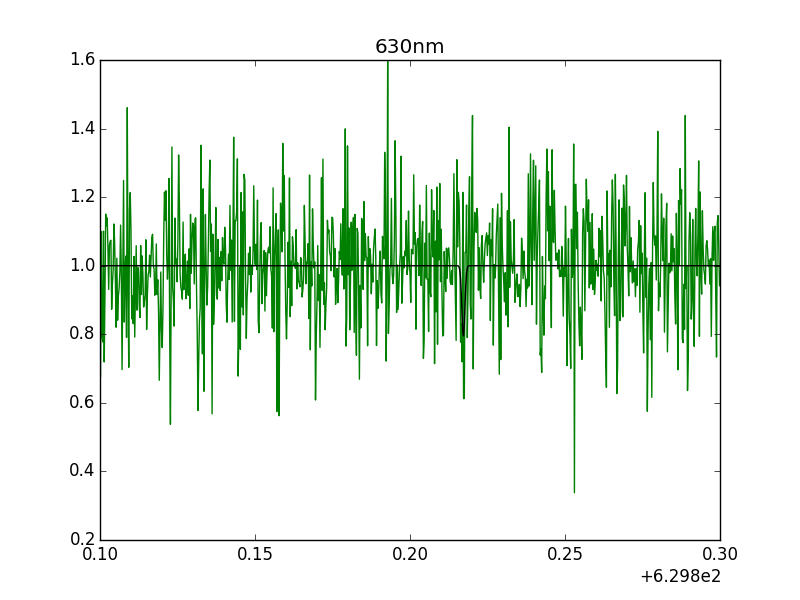
\includegraphics[scale =0.33]{630nm.png}
  \caption{Absoptionline at 630nm}
  \endminipage\hfill
  \minipage{0.32\textwidth}
  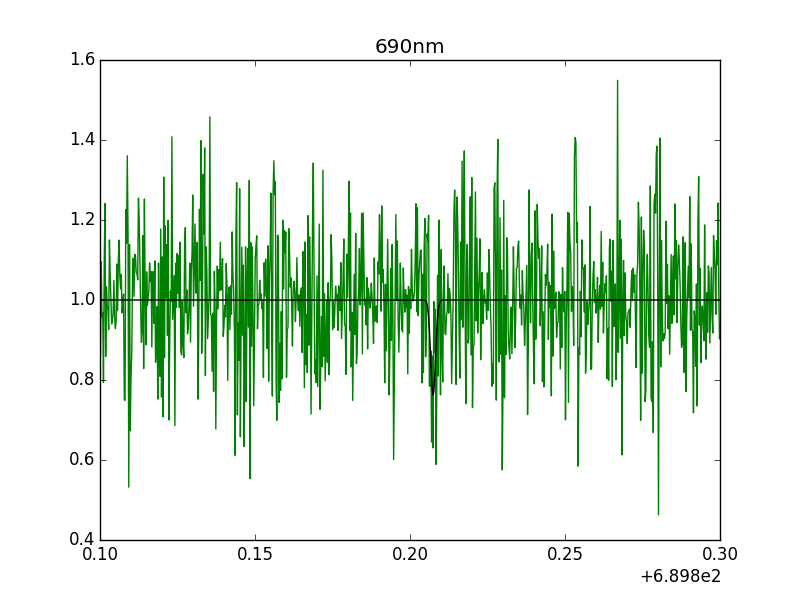
\includegraphics[scale = 0.33]{690nm.png}
  \caption{Absoptionline at 690nm}
  \endminipage\hfill
  \minipage{0.32\textwidth}
  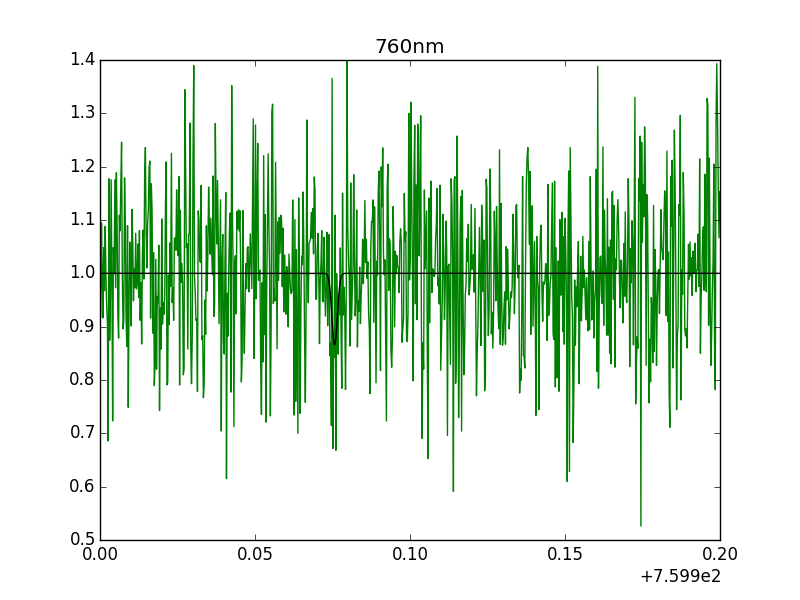
\includegraphics[scale = 0.33]{760nm.png}
  \caption{Absoptionline at 760nm}
  \endminipage
\end{figure}
Where the width black graph is the standard diviation. Looking at the graph, I
see the spectra in the middle stands out. The reason is the width of the graph,
but also  \(F \approx 0.7\) (the flux). Looking at the two other spectra, the diviation is
also small, but flux is around \(0.85-0.87\). This means that Oxygen is very
highly probable to find in the atmosphere. Since the absorptionline at
\(690nm\) have a flux approximated to \(0.7\), I therefore conclude that Oxygen
do exist in the atmosphere.
\newpage
\subsubsection{Methane:} Methane have two absorption lines at \(1660nm\) and
\(2200nm\). The spectra is given down below
\begin{figure}[!htb]
  \minipage{0.4\textwidth}
  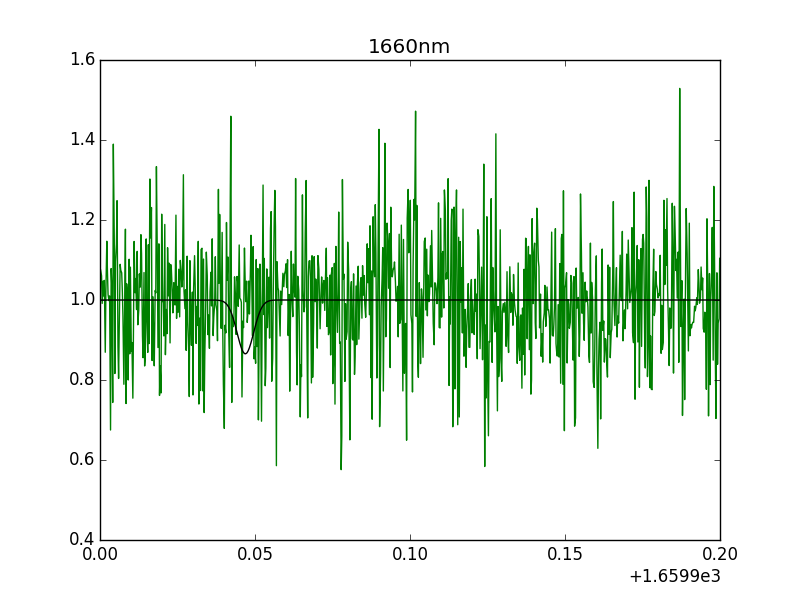
\includegraphics[scale =0.4]{1660nm.png}
  \caption{Absoptionline at 1660nm}
  \endminipage\hfill
  \minipage{0.4\textwidth}
  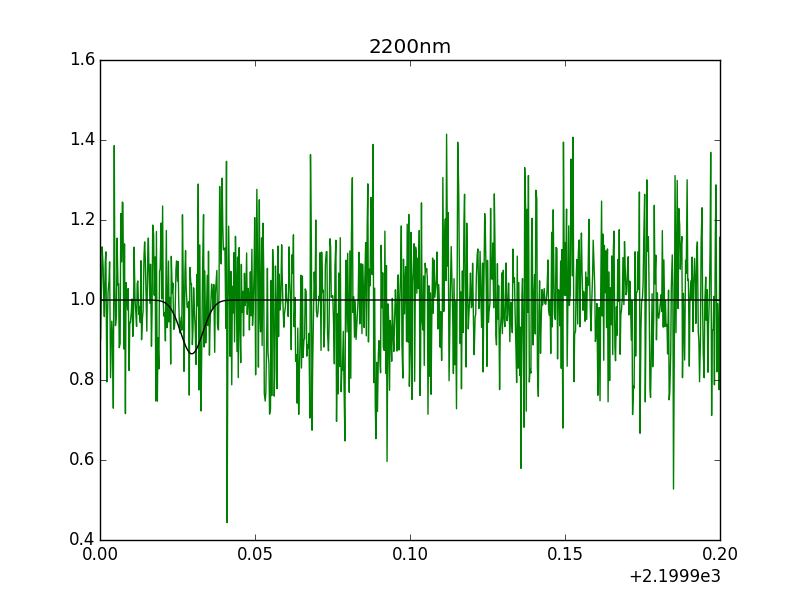
\includegraphics[scale = 0.4]{2200nm.png}
  \caption{Absoptionline at 2200nm}
  \endminipage
\end{figure}
\\
Looking at the spectra, I notice that the standard diviation is quite large,
and the measured is around \(0.9\), which indicates that I caught noise. I
therefore conclude that methane do not exist in the atmosphere.
\subsubsection{Carbon monooxide:} Carbon monooxide have absorptionline at the
wavelength \(2340nm\). The spectra is given down below
\begin{center}
  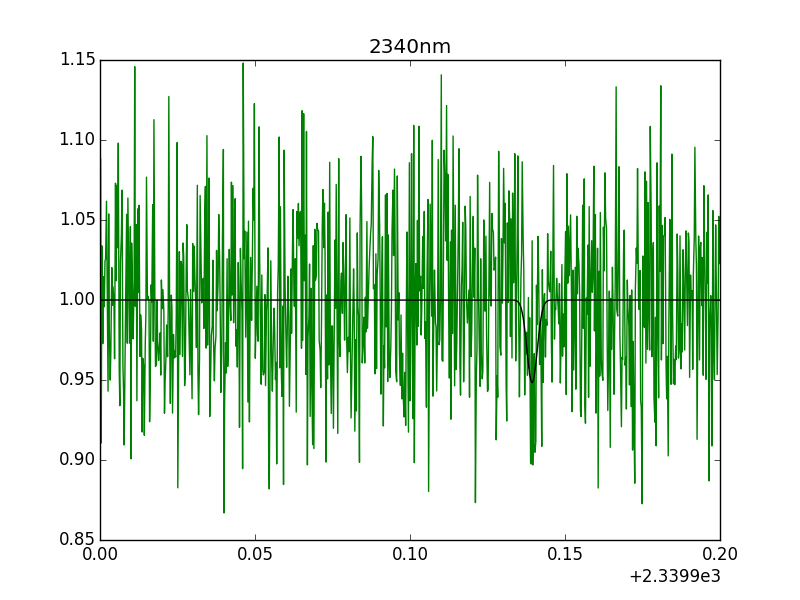
\includegraphics[scale = 0.4]{2340nm.png}
\end{center}
\newpage
Looking at the spectra, I see that the stanard diviation is quite small, but
\(F^{model}\) is around \(0.93-0.96\) which makes me question that I have
detected carbon monooxide. Since the \(F^{model} \approx 1\), I will therefore
conclude that carbon monooxide do not exist in the atmosphere.
\subsubsection{Water vapor:} Water vapor have absorption lines at \(720nm,820nm\)
and \(940\).  
\begin{figure}[!htb]
  \minipage{0.32\textwidth}
  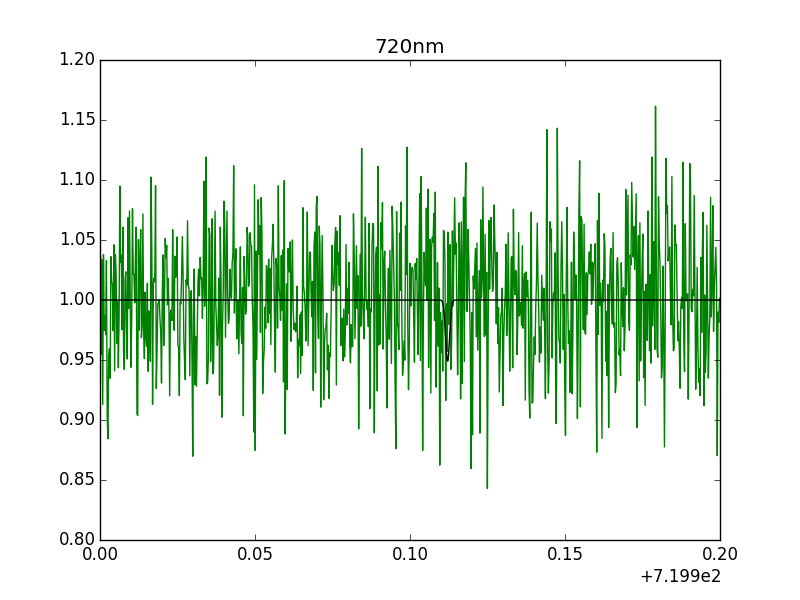
\includegraphics[scale =0.33]{720nm.png}
  \caption{Absoptionline at 720nm}
  \endminipage\hfill
  \minipage{0.32\textwidth}
  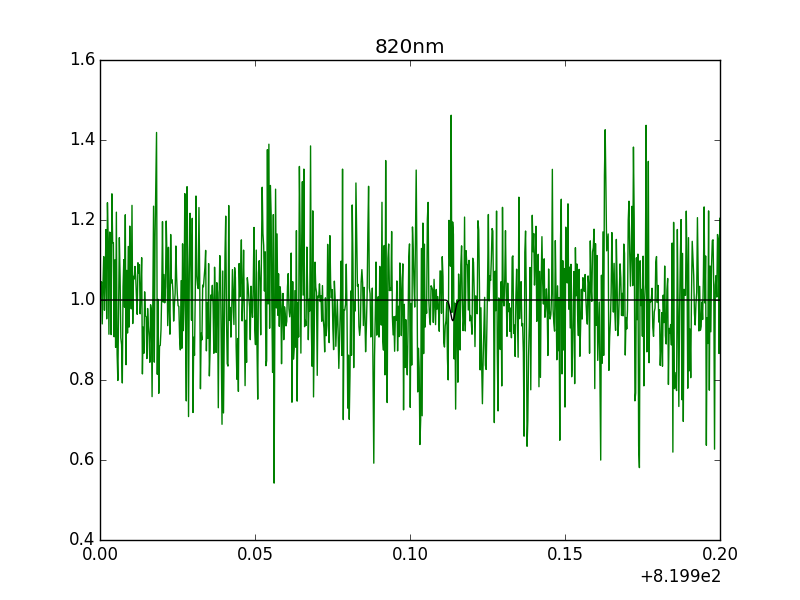
\includegraphics[scale = 0.33]{820nm.png}
  \caption{Absoptionline at 820nm}
  \endminipage\hfill
  \minipage{0.32\textwidth}
  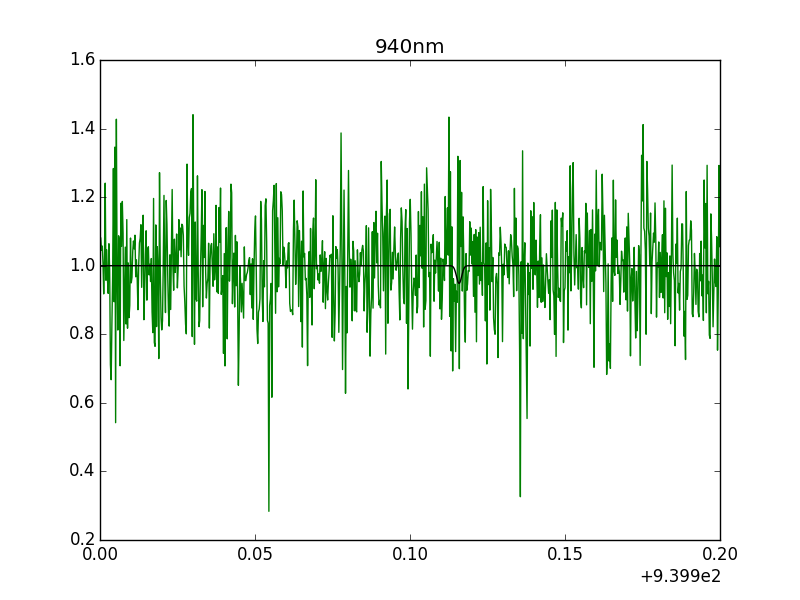
\includegraphics[scale = 0.33]{940nm.png}
  \caption{Absoptionline at 940nm}
  \endminipage
\end{figure}
when looking
at the spectras it looks like that I have not detected water vapor in the
atmosphere. Since all the spectra shows that \(F^{model} \approx 1\), which
means no absorption line.
\subsubsection{Carbon dioxide:} Carbon dioxide have two absoprtionlines at
\(1440nm\) and \(1600nm\).
\begin{center}
  \minipage{0.5\textwidth}
  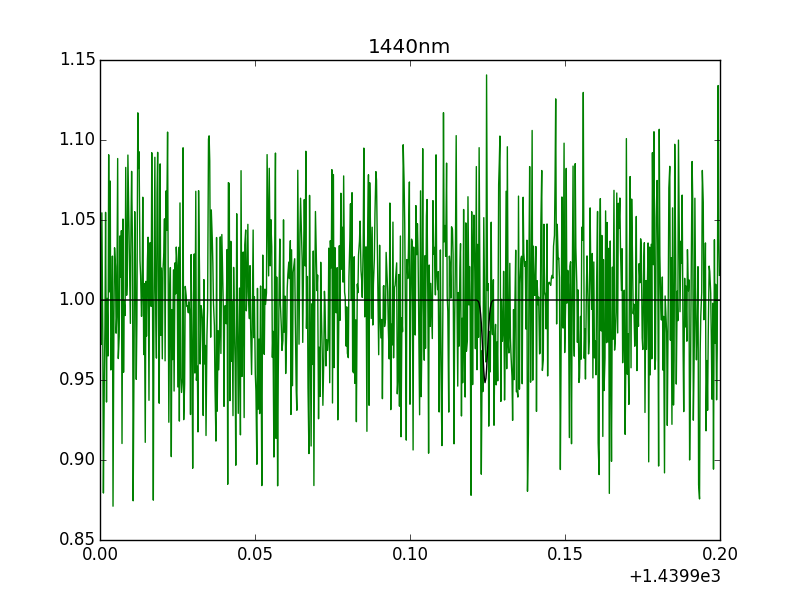
\includegraphics[scale =0.32]{1440nm.png}
  \endminipage\hfill
  \minipage{0.5\textwidth}
  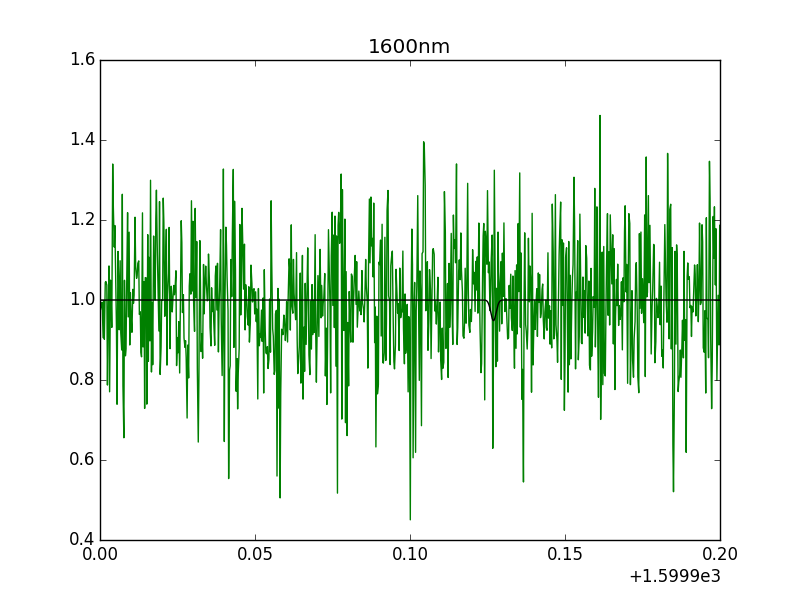
\includegraphics[scale = 0.32]{1600nm.png}
  \endminipage
\end{center}


Looking at the spectra I have not detected any Carbon dioxide in the
atmosphere, even though the standard diviation on the spectra to the left is
small, but \(F^{model} \approx 0.95\) which indicates that I have not detected
carbon monooxide.
\subsubsection{Nitrous oxide:} Nitrous oxide have a absorption line at
\(2870nm\).
\begin{figure}[h]
  \centering
  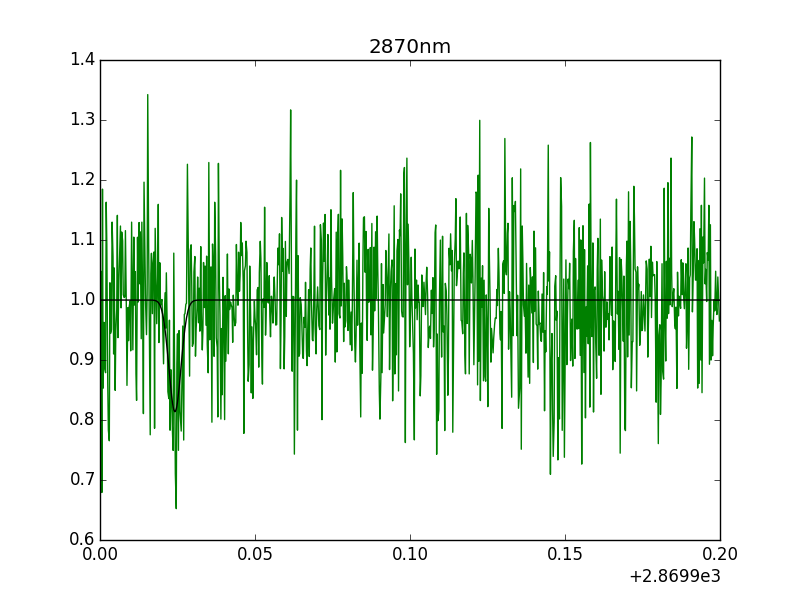
\includegraphics[scale = 0.5]{2870nm.png}
  \caption{A diagram over flux seen and model at the wavelength 2870nm}
\end{figure}
Looking at the spectra it seems that I have detected Nitrous oxide in the
atmosphere, since \(F^{model} \approx\) and have quite small standard divation,
which means this is not noise but a absorption line. I therefore conclude
Nitrous oxide do exist in the atmosphere.
\subsubsection{Conclusion of the data:} Looking through the spectras I
recieved, I conclude that G23's atmosphere highly consist of oxygen and nitrous
oxide. The mean molar mass of G23's atmosphere is
\begin{align}
  \mu_{mean} = 30.00245
\end{align}
\newpage
\subsection{Modeling the atmosphere:} There are several methods to model the
atmosphere. From previous sections I derived a analytical solution of G23
atmosphere, using the mean molar mass \(\mu_{mean} = 30.00245\) the density of
the atmosphere would like
\begin{figure}[h]
  \centering
  \includegraphics[scale = 0.5]{atmosphere.png}
  \caption{A graph showing how the atmosphere changes as the altitude changes}
\end{figure}
\\
Looking at the graph it makes with the calculations done. At the height
\(51.3km\) it will go over to the isothermal part of the atmosphere. Since the
isothermal is exponential function, when the altitude increases the atmospheric
density decreases rapidly. 
\newpage
\mychapter{4}{Conclusion}
\newpage
\mychapter{5}{References}




\end{document}